\chapter{\label{II-B}Partager des structurations similaires de jeux de données par les classes et les propriétés : les ontologies, grammaires communes mais spécifiques}
\titreEntete{Les ontologies, grammaires communes mais spécifiques}

%intro
\lettrine{L}'éclatement des référentiels dans le Web de données conduit à la création, ou au renforcement, de liens entre eux, ainsi qu'entre leurs données. Ces liens doivent porter une valeur sémantique de manière à ce que l'éclatement ait lieu sans perdre d'informations. Il faut alors que le sens des relations soit contrôlé et partagé par le plus grand nombre: les ontologies permettent cela. Ainsi, si le référentiel présenté sous la forme de liste ou de thésaurus disparaît au profit du Web de données, de nouveaux référentiels, adaptés au Web sémantique, prennent le relais.\\

Souvent confondues avec les systèmes organisés de connaissances\footnote{Ils sont fréquemment nommés KOS pour \textit{Knowledge Organization Systems}.}, les ontologies diffèrent par leur formalisme. La \reference{controler} a montré qu'une interopérabilité par les référentiels est possible et que les arbres de classification portent difficilement du sens, l'arborescence permettant essentiellement d'effectuer une classification; avec les ontologies, une interopérabilité sémantique peut avoir lieu.\\

De même qu'avec le Web de données, le milieu bibliothéconomique a été l'un des premiers à adopter massivement les ontologies afin de pouvoir typer les relations entre les entités: l'ontologie est essentielle au Web sémantique.\\

\section{\label{II-B-1}L'ontologie, un vocabulaire structurant}
\titreEntete{L'ontologie, un vocabulaire structurant}

%intro
Dans le chapitre précédent\footnote{Voir \reference{II-A}.}, nous avons évoqué un premier type de référentiel --- les vocabulaires de valeurs --- présent dans le Web de données. De manière à pouvoir décrire ces ressources\footnote{\og L'une des fonctions des ontologies est de permettre de définir la nature des ressources\fg{} in \cite[§49]{bermes_convergence_2013}.}, d'autres référentiels sont nécessaires, les ontologies, en fournissant les classes et les propriétés utiles aux descriptions. Au-delà de l'apport de ces éléments, l'ontologie permet également une description formelle par des axiomes et des règles de raisonnement, visibles dans le Web de données avec \ac{rdfs} et \ac{owl}.\\

L'\index[ref]{typologie@Typologie!ontologie@Ontologie}ontologie informatique est un concept récent, né à la fin du \textsc{XX}\textsuperscript{ème}siècle comme le Web. Plusieurs types d'ontologies existent, reflétant leur caractère universel ou non, leur domaine de description; leur structuration et leur formation doivent cependant répondre à des critères précis de manière à structurer le plus efficacement possible des référentiels.

\subsection{\label{II-B-1-a}Origines de l'ontologie informatique}
\titreEntete{Origines de l'ontologie informatique}

\begin{citationLongue}
	[Les ontologies sont] des vocabulaires de termes --- classes, relations, fonctions, constantes d'objet --- avec des définitions communes, sous la forme d'un texte compréhensible par les humains et applicable à la machine, de contraintes déclaratives dans leur forme la mieux formée.\footnote{\og vocabulaires of representational terms --- classes, relations, functions, object constants ---  with agreed-upon definitions, in the form of human-readable text and machine-enforceable, declarative constraints on their well formed use\fg{} in \cite[p.2]{gruber_role_1991}}
\end{citationLongue}

\index[ref]{typologie@Typologie!ontologie@Ontologie}L'ontologie est d'abord une science philosophique, née avec les \textit{Catégories} d'Aristote, étudiant la réalité des entités, les relations qu'elles entretiennent --- hiérarchie, similarité --- pour trouver les similarités et les différences présentes dans le monde. Au \textsc{XIX}\textsuperscript{ème}siècle, le siècle de la \index[ref]{typologie@Typologie!taxonomie@Taxonomie}taxonomie, cette science philosophique devient l'étude de l'ensemble des connaissances existantes dans le monde\footcite{welty_supporting_2011}.\\

Ce n'est qu'en 1991\footcite{gruber_role_1991}, puis 1993\footcite{gruber_toward_1993}, que \nP{Thomas R.}{Gruber}, souhaitant améliorer l'intelligence artificielle et l'indexation structurée, évoque l'ontologie informatique, pensée comme un ensemble déclaratif d'entités, destinée au partage des connaissances entre les machines: \og Une ontologie est une spécification explicite d’une conceptualisation\fg{}\footnote{\og An ontology is an explicit specification of a conceptualization. \fg{} in \cite[p.1]{gruber_toward_1993}.}. Cette définition, donnée très tôt par \nP{Thomas R.}{Gruber}, permet d'observer deux principes de l'ontologie: premièrement, elle est une conceptualisation d'un domaine, par conséquent elle est un choix de description sur un domaine précis; deuxièmement, cette conceptualisation est spécifiée, c'est à dire qu'elle a une description formelle.\\

\nP{Rudi}{Studer} apporte des précisions en 1998\footcite{studer_knowledge_1998} en proposant une nouvelle définition plus spécifique de \index[ref]{typologie@Typologie!ontologie@Ontologie}l'ontologie: \og Une ontologie est
une spécification formelle et explicite d’une conceptualisation partagée\fg{}\footnote{\og An ontologyis a formal, explicit specification of a shared conceptualization\fg{} in \cite{studer_knowledge_1998}}. Une ontologie est formelle de manière à pouvoir être comprise par une machine; elle est une spécification explicite par la déclarativité de ses concepts, de ses propriétés, \dots~; elle est partagée car elle prend l'ensemble des connaissances d'une communauté, d'un domaine; enfin, la conceptualisation renvoie au domaine décrit par cette ontologie.\\

\index[ref]{typologie@Typologie!ontologie@Ontologie}L'ontologie est un référentiel de classes et de propriétés, ne s'appliquant qu'à un seul domaine particulier de la connaissance, mais permettant de le structurer. Son fort développement a permis une application dans le Web de données et dans le milieu bibliothéconomique qui considère les ontologies comme \og des éléments de description de métadonnées\fg{}\footcite{baker_rapport_2012}.

\subsection{\label{II-B-1-b}Des ontologies différentes}
\titreEntete{Des ontologies différentes}

Il existe une grande diversité \index[ref]{typologie@Typologie!ontologie@Ontologie}d'ontologies. Certaines sont plus importantes que d'autres du fait du nombre d'utilisations qu'elles entraînent et de leur généralité; d'autres, plus spécifiques, paraissent moins importantes par le faible nombre de liens qu'elles suscitent. Les ontologies peuvent également être classées selon les usages qui en sont faits, que leur finalité soit une publication sur le Web sémantique ou simplement une utilisation interne à une institution.\\

Au plus haut niveau se trouvent des ontologies \og noyaux\fg{}\footcite[p.4]{isaac_les_2012} qui modélisent les connaissances communes,, partageables et réutilisables d'un domaine à un autre: le modèle \index[ref]{modelisation@Modélisation!cidoc@CIDOC-CRM}\ac{cidoccrm} des musées propose ainsi une ontologie réutilisée dans \index[ref]{relier@Relier!rdfs@RDFS}\ac{rdfs} notamment\footnote{Voir \reference{annexe_onto} (\reference{onto_crm}).}. Son vocabulaire correspond aux événements, aux objets, aux moments, \dots ~ ce qui en fait un vocabulaire générique pour d'autres ontologies de plus bas niveau.\\

Au niveau inférieur se trouvent les \index[ref]{typologie@Typologie!ontologie@Ontologie}ontologies de domaine, propres à un domaine en particulier: elles modélisent les connaissances de ce domaine uniquement; elles offrent des concepts et des relations permettant de décrire les activités et les vocabulaires du domaine en question. Les concepts de ces ontologies de domaine sont souvent des spécialisations\footnote{Ainsi que le faisait remarquer \nP{Rudi}{Studer} en 1998 in \cite{studer_knowledge_1998}.} d'ontologies de plus haut niveau. L'ontologie \index[ref]{modelisation@Modélisation!frbr@FRBR}\index[ref]{relier@Relier!frbr@FRBR}\ac{frbr}\footnote{Décrite dans la \reference{II-B-3}.} peut être considérée comme une de ces ontologies de domaine car elle utilise \ac{rdfs}, les \index[ref]{relier@Relier!dcterms@DC Terms}\textit{Dublin Core Terms} (DC Terms), et d'autres ontologies de haut niveau\footnote{Voir \reference{annexe_onto} (\reference{onto_frbr})}.\\

Plus bas encore, il existe des ontologies utilisées, par un petit nombre d'utilisateurs, dans l'unique cadre d'utilisations applicatives. Elles ne modélisent par conséquent que les termes et les relations nécessaires à l'application, en utilisant principalement des ontologies de plus haut niveau, notamment celles de domaine\footnote{L'ontologie \index[ref]{relier@Relier!c4o@C4O}\textit{Citation Counting and Context Characterization Ontology}(C4O) est l'une de ces ontologies applicatives, ayant peu d'ontologies l'utilisant, et utilisant un grand nombre d'ontologies de plus haut niveau. Voir \reference{annexe_onto} (\reference{onto_c4o}).}.\\

De multiples \index[ref]{typologie@Typologie!ontologie@Ontologie}ontologies existent et diffèrent de cette hiérarchisation\footcite[p.2]{isaac_les_2012} et participent à la diversité des ontologies. Cette diversité est essentielle pour décrire tout type d'objets ou d'événements --- que ce soit dans le milieu culturel ou non ---, ou pour relier à ces ontologies des vocabulaires propres: elle participe à l'interopérabilité des référentiels entre eux. Cette interopérabilité, grâce aux ontologies, peut être entre un système documentaire interne et le Web de données, ou bien entre deux jeux de données du même Web de données.

\subsection{\label{II-B-1-c}Les principes de l'ontologie}
\titreEntete{Les principes de l'ontologie}

Permettre l'interopérabilité entre tout type de données et de jeux de données nécessite une structure et des principes. Dans la publication de 1993\footcite{gruber_toward_1993}, \nP{Thomas R.}{Gruber} édicte déjà cinq critères sans lesquels une \index[ref]{typologie@Typologie!ontologie@Ontologie}ontologie ne peut pas être formée correctement. Ces critères généraux contraignent la graphie tout en laissant le champ ouvert aux modifications futures d'une ontologie. Il préconise ainsi:
\begin{itemize}
	\item la clarté des termes décrits: leur description doit être objective, complète, et réalisée dans le langage naturel;
	\item la cohérence des axiomes retenus et l'interdiction de la discordance entre les termes et les axiomes: elle permet la spécialisation de la conceptualisation qui est la définition de l'ontologie;
	\item la possibilité d'étendre l'ontologie même après sa création: cela permet d'accepter les changements d'usages ou de besoins liés à cette ontologie, et par conséquent de la faire évoluer facilement;
	\item le biais d'encodage doit être minimal de manière à permettre la plus grande interopérabilité;
	\item l'engagement dans l'ontologie doit être minimal, les termes utilisés doivent être ceux les plus souvent utilisés: cela permet la réutilisation de l'ontologie
\end{itemize}
\bigskip

Ces cinq critères \index[ref]{typologie@Typologie!ontologie@Ontologie}ontologiques dirigent la structure et la nature des éléments essentiels aux ontologies et les constituant. Les concepts sont le premier de ces éléments: ils permettent de définir des idées, des objets ou des notions. De même que pour les \index[ref]{typologie@Typologie!vocabulaires controles@Vocabulaires contrôlés}vocabulaires contrôlés\footnote{Voir \reference{I-A-2}.}, plusieurs propriétés peuvent s'appliquer à ces concepts. \nP{Nicola}{Guarino} décrit ces propriétés\footcite{guarino_formal_1998} de généricité --- absence d'extension pour le concept ---, d'identité, de rigidité --- si une instance du concept reste en permanence son instance ---, d'anti-rigidité --- si une instance est principalement définie par son appartenance à un autre concept --- et d'unité des concepts. Ainsi, deux concepts peuvent être disjoints, équivalents ou dépendants.\\

Les relations sont une autre partie essentielle des ontologies, sans lesquelles les concepts n'ont pas de sens entre eux et ne peuvent être formalisés. Elles peuvent être inclusives --- hiérarchiques ---, ou ensemblistes avec des unions, des intersections ou des exclusions. À ces relations peuvent d'ajouter des axiomes, des règles, qui viennent régir les contraintes, les relations ou les concepts eux-mêmes.\\

Les différents principes des \index[ref]{typologie@Typologie!ontologie@Ontologie}ontologies les rendent strictes sur leur formation et leur structure, de nombreuses propriétés s'imposant. Complexes, ils permettent néanmoins la création d'un vocabulaire à la fois contrôlé, hiérarchique et utilisable par tous.

%conclu
\bigskip
\bigskip
L'ontologie peut alors trouver son intérêt sur le Web avec une indexation réalisée par les moteurs de recherche; sur le Web et en institution en permettant la description de jeux de données par des ontologies publiques; en structurant la connaissance du monde. La principale application est bibliothéconomique avec la possibilité de valoriser et de publier les collections sous forme de métadonnées. Enfin, l'ontologie permet de relier deux jeux de données, deux référentiels, pourtant éloignés, selon un vocabulaire commun partagé publiquement.
\section{\label{II-B-2}Des \textit{Knowledge Organization Systems} (KOS) à \ac{skos}: vers l'interopérabilité syntaxique}
\titreEntete{Vers l'interopérabilité syntaxique}

%intro
Les ontologies ressemblent fortement aux \textit{thesauri} et autres vocabulaires contrôlés --- les \ac{kos} --- à cause du contrôle de la graphie, des termes retenus ou rejetés, et de l'établissement de relations entre les termes. Cependant, une ontologie n'est pas nécessairement un thésaurus, alors qu'un thésaurus est une ontologie. Bien que la distinction entre les deux soit mince, elle est essentielle en raison du formalisme qui compose les ontologies.\\

L'interopérabilité sémantique permise par les ontologies bâtit de l'interconnexion entre les jeux de données, rend possible l'échange et la publication de données nativement différentes sur le Web de données. La conversion par les institutions patrimoniales d'une partie ou de l'ensemble de leurs vocabulaires en ontologies a été permise par l'ontologie \ac{skos}.

\subsection{\label{II-B-2-a}Distinguer les systèmes d'organisation de la connaissance des ontologies}
\titreEntete{Distinguer les KOS des ontologies}

Les \ac{kos} sont des référentiels contrôlés de vedettes et de termes qui ne sont valables que pour un domaine d'activité et de la connaissance. Ils sont souvent organisés par des relations terminologiques et sémantiques qui les font se confondre avec les ontologies en raison de leur formalisation\footcite[p.48]{dalbin_approches_2011}. Plus encore, sur le Web de données, les \ac{kos} ne jouent pas de rôle, ils n'apportent pas de structure, mais complètent des référentiels ou des jeux de données déjà existants. Les \ac{kos} n'offrent qu'une succession de termes destinés à remplir des champs descriptifs, alors que les ontologies dirigent directement les données et leur structure.\\

Les ontologies permettent de dépasser certaines limites des \ac{kos} relevées dans la \reference{controler}\footcite{isaac_les_2012}:
\begin{itemize}
	\item les \textit{thesauri} et autres vocabulaires sont destinés d'abord à un utilisateur humain qui peut facilement comprendre la structure du vocabulaire\footnote{C'est le cas de la visualisation graphique du thésaurus des noms communs de l'\ac{ina}. Voir \reference{annexe_thesaurus} (\reference{thesaurus_cadreur}).}; les ontologies visent quant à elles à d'abord être comprises par une machine et le Web sémantique;
	\item les \ac{kos} induisent souvent des relations diverses et variables, notamment dans le cas de relations génériques--spécifiques
\end{itemize}
\medskip
Les limites identifiées sont dues principalement aux relations des termes des \ac{kos}: ces vocabulaires ne sont pas sémantiques, seulement hiérarchiques dans le but de classer et d'aider l'humain dans la compréhension du contexte du terme. L'apport des ontologies est l'ajout de sens aux termes grâce aux relations qu'ils entretiennent entre eux.


\subsection{\label{II-B-2-b}\ac{skos}: exposer les systèmes d'organisation de la connaissance sur le Web de données}
\titreEntete{SKOS: exposer les KOS sur le Web de données}

Dans le but de permettre aux institutions d'établir des liens entre leurs référentiels et leurs données, \ac{skos} a été créé. \ac{skos} est \og une ontologie qui se veut simple et compatible avec une majorité d’approches d’organisation des connaissances existantes (thésaurus, classifications\dots)\fg{}\footcite[p.8]{isaac_les_2012}. Elle permet de représenter presque tous les types de vocabulaires en concepts liés. \ac{skos} n'est pas un référentiel, seulement un moyen de faciliter l'interconnexion entre les données, leur échange, et de créer de nouveaux usages jusqu'alors impossibles.\\

Pour cela, \ac{skos}, vocabulaire \ac{rdf}, reprend les propriétés des vocabulaires contrôlés, notamment du thésaurus. En effet, il est possible d'indiquer des termes préférentiels, alternatifs, traduits, variants, \dots~;de plus, des notes peuvent être introduites; enfin, des liens --- génériques et hiérarchiques, associatifs, \dots~ sont créés entre les différents concepts\footnote{Voir \reference{skos_modelisation}.}. \ac{skos} a le rôle de l'essieu dans le modèle de l'interopérabilité de la roue et de l'essieu. Elle offre un petit nombre de concepts servant à la description et à la transcription d'un thésaurus dans un langage compréhensible par une machine. Ainsi, \ac{skos} est une ontologie de domaine: elle hérite d'autres ontologies comme DC Terms ou \ac{rdfs}, et sert d'ontologie de haut niveau pour des ontologies de plus bas niveau\footnote{La consultation de \url{https://lov.linkeddata.es/dataset/lov/vocabs/frbr} permet de constater ce rôle pivot de \ac{skos} pour les autres ontologies, ainsi que sa dépendance à d'autres ontologies.}.\\

\begin{figure}[!h]
	\centering
	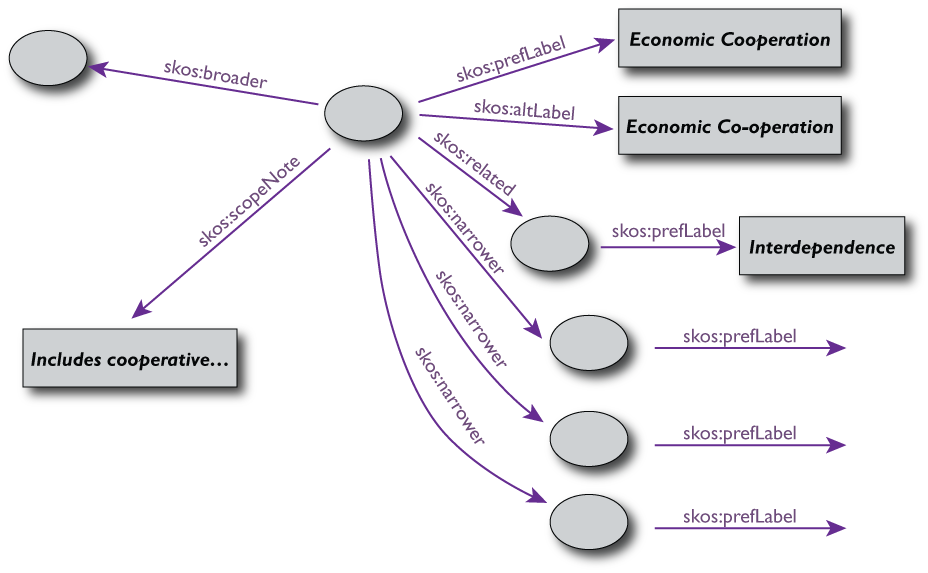
\includegraphics[width=13cm]{images/SKOS_simpleThesaurus.png}
	\caption[Modélisation simplifiée de \ac{skos}]{Modélisation simplifiée de \ac{skos} [Source: \href{https://www.w3.org/Consortium/Offices/Presentations/RDFTutorial/figures/SKOS_simpleThesaurus.png}{www.w3.org}]}
	\label{skos_modelisation}
\end{figure}
\medskip

Enfin, des propriétés de \ac{skos} permettent de créer du lien entre des concepts provenant de différentes sources: ce sont les propriétés d'équivalence ou de similitude <skos:broader>, <skos:exactMatch> ou <skos:closeMatch>. Ces propriétés permettent le rapprochement de plusieurs concepts: le \ac{lcsh}\footnote{Voir \reference{lcsh_liens}.} peut ainsi utiliser \ac{skos} pour créer des fiches de liens. De même, la Bibliothèque nationale de France (BnF) contient des références à l'ontologie Dewey qui lui permet ainsi d'obtenir des relations d'équivalence avec ses données. Alors, l'emploi de \ac{skos} nécessite des URIs de manière à créer des triplets \ac{rdf}.\\

Avec \ac{skos}, l'interopérabilité sémantique est désormais possible entre les institutions sur le Web de données. Cette ontologie \ac{rdf} permet de rapprocher des jeux de données et des référentiels jusqu'alors séparés et pourtant similaires. Le vocabulaire offert pour décrire les \textit{thesauri} et ensuite les partager dans le Web sémantique permet de nombreuses applications en institutions, et facilite ainsi les opérations d'indexation ou de recherche.

%conclu
\bigskip
\bigskip
Cependant, les vocabulaires des institutions n'étant pas nativement liés entre eux, il reste difficile de les aligner, et par conséquent de passer d'un \ac{kos} à une modélisation \ac{skos}, notamment pour les relations partie--tout. \nP{Sylvie}{Dalbin} prend en exemple\footcite{dalbin_approches_2011} ce type de relation qui peut être exprimé dans le Web sémantique par trois types de relations: hiérarchique, instance--classe, ou bien sous-classe--classe. Ces incertitudes rendent le processus d'ontologisation complexe, qui l'est d'autant plus quand les termes sont dans des langues différentes.\\

Les ontologies apparaissent comme un référentiel essentiel dans le Web de données, plus encore que les autorités qui sont devenues des données; elles ont permis l'apparition d'un Web sémantique. Seulement, la problématique de l'alignement de référentiels entre eux sur le Web de données est toujours présente et ne sera jamais totalement résolue.
\section{\label{II-B-3}Les ontologies dans le Web sémantique}
\titreEntete{Les ontologies dans le Web sémantique}

%intro
La finalité principale des ontologies est leur exposition sur le Web de données. L'utilisation qui s'ensuit permet la création d'un Web sémantique, structuré et aux données partagées. Le référentiel compris dans le sens de \ac{kos} n'intervient plus autant dans ce Web sémantique; le modèle de description de ces référentiels s'impose sous la forme des ontologies et améliore dans le même temps la description des concepts qu'il contient par des relations typées.\\

Cette avancée permet une description plus fine et partagée des documents des institutions patrimoniales: le référentiel est à la fois leur propres données et celles du Web de données, liées par les ontologies publiques.

\subsection{\label{II-B-3-a}Décrire des ontologies en \ac{rdf}: \ac{rdfs} et \ac{owl}}
\titreEntete{Décrire des ontologies en RDF}

De même que \ac{skos} est une ontologie permettant la description de \ac{kos}, \ac{rdfs} et \ac{owl} sont les représentations des ontologies \ac{rdf}. Les documents décrits par les institutions le sont par des formats et des logiques différentes. Utiliser une seule ontologie peut s'avérer difficile; en effet, elle peut être trop large ou trop spécifique pour le domaine décrit. C'est pourquoi l'utilisation des URIs, des liens hypertexte du Web, permet d'utiliser autant d'ontologies que nécessaire, et de créer une interopérabilité par parcours de liens, par rebonds sur les URIs.\\

La constitution de ce réseau de liens utilisé pour la description de documents n'est possible qu'avec l'utilisation du Web sémantique et de \ac{rdf}. C'est pourquoi il a été nécessaire de construire des modèles de représentation des ontologies en \ac{rdf}.\\

\ac{rdfs} est un langage de description simple, destiné à apporter les bases d'une description en \ac{rdf} avec la déclaration de classes --- et de sous-classes --- et de propriétés. Les classes sont des concepts, des types de ressources, identifiés par des URIs. Les propriétés sont les relations qui existent entre les classes. Ainsi, chaque ressource est instanciée à une classe par la propriété --- le prédicat \ac{rdf} --- <http://www.w3.org/1999/02/22-rdf-syntax-ns\#type> (rdf:type). La présence de sous-classes permet de créer des groupes au sein de classes: en déclarant une instance d'une sous-classe, un second triplet est alors implicitement créé entre la sous-classe et la classe avec le prédicat rdfs:subClassOf. Tout ce qui s'applique à une classe est appliqué à une sous-classe.\\

\ac{rdfs} admet aussi la déclaration de domaines et de codomaines pour les propriétés. Ces propriétés peuvent être de type ressource quand elles relient deux ressources désignées par des URIs, ou bien de type donnée quand l'objet est un littéral. Ce comportement des propriétés est déclaré avec le domaine et le codomaine: le domaine de la propriété définit la type de la classe sujet, tandis que le codomaine définit la classe de la ressource objet --- ou du type de donnée si c'est un littéral.\\

Malgré les classes et sous-classes, et les domaines et codomaines, \ac{rdfs} reste simple et ne permet pas de description complexe de relations. C'est pourquoi \ac{owl} est une extension de \ac{rdfs}. Des contraintes sur les relations comme la symétrie, l'équivalence, la différence ou la contradiction peuvent être exprimées; de même, la déclaration d'une liste d'instances contrôlées peut être faite. Comme avec \ac{skos}, il est possible, et souvent indispensable, de déclarer des relations d'équivalences entre les classes, les propriétés ou les instances. Ainsi, une instance peut hériter des propriétés de la classe à laquelle sa classe est équivalente. Pour cela, trois propriétés \ac{owl} existent: <http://www.w3.org/2002/07/owl\#equivalentClass> (owl:equivalentClass), <http://www.w3.org/2002/07/owl\#equivalentProperty> (owl:equivalentProperty) et <http://www.w3.org/2002/07/owl\#sameAs> (owl:sameAs).

\subsection{\label{II-B-3-b}Utilisation des ontologies en institutions}
\titreEntete{Utilisation des ontologies en institutions}

Chaque ontologie traitant d'un domaine particulier de la connaissance ou du monde, elles sont très nombreuses. Dans sa constante réflexion sur la description, l'indexation et le partage de ses données, le milieu bibliothéconomique s'est emparé du Web de données pour faciliter ses missions et la recherche. Ainsi, plusieurs ontologies sont essentielles dans ce milieu. La première, DC Terms\footcite{noauthor_dublin_nodate}, et la plus ancienne car créée en 1995, permet la description bibliographique d'un document sur le Web avec quinze propriétés, accompagnées de propriétés affinées --- \textit{abstract} l'est de \textit{description}. L'ontologie Dublin Core est constamment utilisée en bibliothèques\footnote{La \reference{onto_dcterms} montre la quantité d'ontologies l'utilisant.}, et plus généralement dans le Web de données, car elle offre les outils de base servant à la description d'un document.
\begin{figure}[!h]
	\centering
	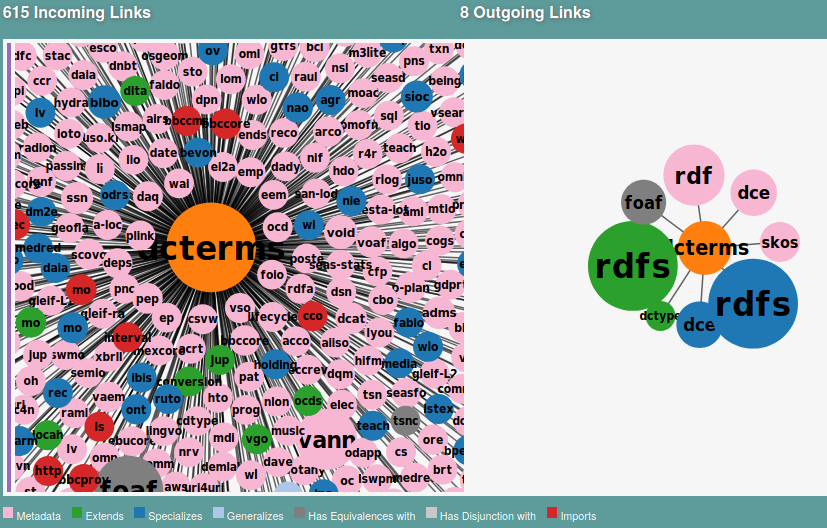
\includegraphics[width=13cm]{images/onto_dcterms.png}
	\caption[L'ontologie DC Terms]{DC Terms: représentation des ontologies l'utilisant (à gauche) et de celles qu'elle utilise(à droite) [Source: \url{https://lov.linkeddata.es/dataset/lov/vocabs/dcterms}]}
	\label{onto_dcterms}
\end{figure}
\medskip

Pour la description des autorités, l'ontologie \ac{foaf}\footcite{noauthor_foaf_nodate} est disponible et est également fortement utilisée. Créée au milieu des années 2000, elle permet la description des agents, de groupes et d'organisations, de personnes, mais aussi de réseaux sociaux.\\

Les ontologies propres aux institutions patrimoniales utilisent ces ontologies de haut niveau. Ainsi, \ac{bibo} utilise à la fois les DC Terms et \ac{foaf}. \ac{cidoccrm}\footnote{Voir \reference{annexe_onto} (\reference{onto_c4o})}, contrairement aux autres ontologies institutionnelles, n'est pas de bas niveau, mais de haut niveau. En effet, elle souhaite pouvoir décrire n'importe quel type d'objet: elle dispose de quatre-vingt-cinq classes et de plus de deux cent cinquante propriétés.

%conclu
\bigskip
\bigskip
\bigskip
Les \index[ref]{modelisation@Modélisation!frbr@FRBR}\index[ref]{relier@Relier!frbr@FRBR}\ac{frbr} et le modèle de données de la BnF permettent de conclure sur l'importance, pour les institutions, des ontologies dans le Web de données. En effet, son modèle de données étant basé sur les \ac{frbr}, tous les types de relations sont nécessaires pour relier l'œuvre aux points d'accès --- autorités, sujets, dates, \dots~ Ces relations sont exprimées par des ontologies publiques: l'exposition \index[ref]{echanges@Échanges!formats@Formats!rdf@RDF}\ac{rdf} des données permet alors l'utilisation des URIs des ontologies ainsi que la description fine du document décrit et de son contexte. Treize ontologies sont ainsi utilisées\footnote{Voir \reference{mdd_bnf}.}, uniquement partiellement pour les propriétés nécessaires à la BnF:
\begin{itemize}
	\item \index[ref]{relier@Relier!foaf@FOAF}\ac{foaf} pour les autorités;
	\item \index[ref]{echanges@Échanges!formats@Formats!rdf@RDF}\ac{rdf} pour exprimer les instances --- avec rdf:type ---;
	\item \index[ref]{relier@Relier!rdfs@RDFS}\ac{rdfs}
	\item \index[ref]{relier@Relier!skos@SKOS}\ac{skos} pour créer le concept préférentiel et définir les sujets proches 
	\item \index[ref]{relier@Relier!dcterms@DC Terms}DC Terms pour les descriptions bibliographiques simples
	\item Geo pour les descriptions géographiques
	\item \index[ref]{echanges@Échanges!formats@Formats!rda@RDA}\index[ref]{relier@Relier!rda@RDA}FRBR-RDA, RDAgroup2elements et RDArelationships pour exprimer les entités du modèle \ac{frbr}
	\item des ontologies internes, BNF-onto et BNFroles
	\item l'extension \ac{rdf} \index[ref]{relier@Relier!owl@OWL}\ac{owl}-time
	\item enfin une ontologie du langage de catalogage \ac{marc} MARCrel
\end{itemize}

L'exemple de la BnF montre qu'il n'y a plus de référentiel unique propre à une institution, mais seulement un ensemble de données dispersées dans le Web de données --- utilisation de \ac{rameau} notamment --- avec des ontologies qui permettent la production de sens sur les liens entre les ressources.\\

\begin{figure}[!h]
	\centering
	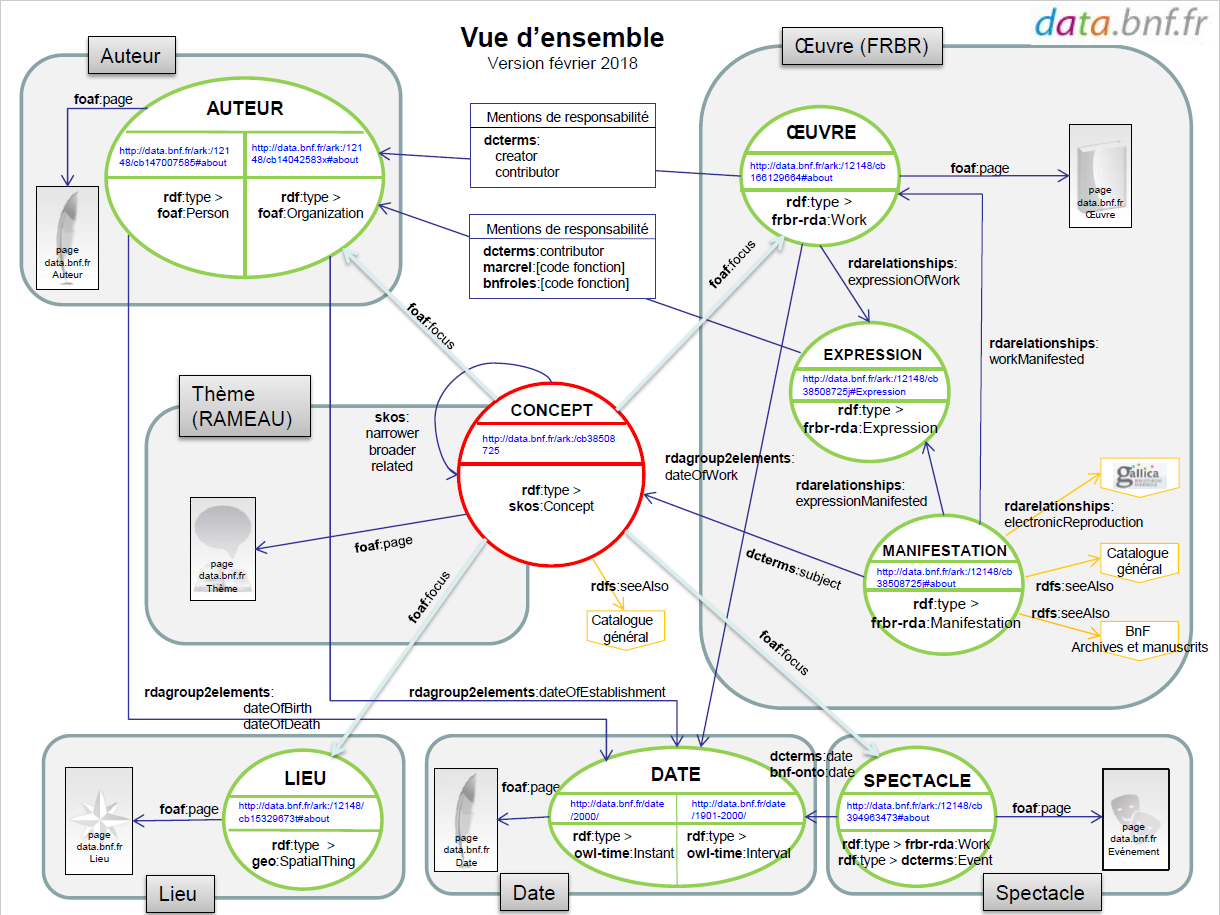
\includegraphics[width=15cm]{images/mdd_bnf.PNG}
	\caption[Le modèle de données de la BnF]{Le modèle de données de la BnF [Source: \url{https://data.bnf.fr/images/modele_donnees_2018_02.PNG}]}
	\label{mdd_bnf}
\end{figure}